\section{FEATURE EXTRACTION}
The framework is developed to acquire time series data from an arbitrary configuration of sensors. When a time series is available, the FA extracts the features. Each time series is linked to a specific set of features to be extracted.

\subsection{Feature set}
The considered features are divided into two categories:
\begin{itemize}
    \item \textbf{Time domain features}: Mean, Standard deviation, Peak-to-peak value (P2P), Root Mean Square value (RMS), Skewness and Kurtosis.
    \item \textbf{Frequency domain features}: Energy of the Wavelet Packet Decomposition (WPD) coefficients, Fast Fourier Transform (FFT) coefficients. The WPD is based on the PyWavelets\footnote{\url{https://github.com/PyWavelets/pywt.git}} and Wavelib\footnote{\url{https://github.com/rafat/wavelib.git}} libraries.
\end{itemize}

The time domain features are computed in the corrected form for sampled data. In the frequency domain, the WPD is preferred in this work, because it reduces the dimensionality of the feature space. The features are standardized along the training dataset so that the mean and standard deviation are 0 and 1, respectively. This is done to ease the training of the UML algorithms.

\subsection{Scaling and selection}
\begin{figure}
    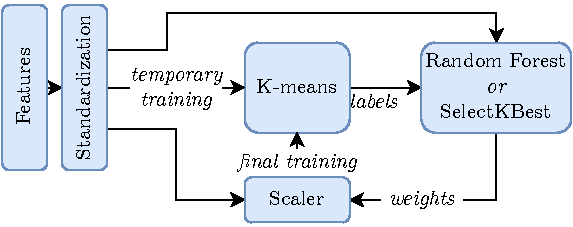
\includegraphics[width=\linewidth]{images/Feat_scaling.pdf}
    \caption{Feature scaling and selection procedure. The features are standardized and then scaled by a weight array or selected to reduce the feature space dimensionality, discarding the less informative features.}
    \label{fig:feature_scaling}
\end{figure}
Despite the standardization, during the experimental validation, it has been observed that some features are more informative than others. To reduce the impact of the less informative features, an optional feature scaling and selection step can be performed, as shown in Fig.~\ref{fig:feature_scaling}. The weights used for scaling the features can be computed by performing a Random Forest training or using the SelectKBest library method.